\documentclass{article}
\usepackage{tikz}

\tikzset{%
    simple node/.style = {%
        rectangle, draw%
    },
    barred node/.style = {%
        simple node,% 
        path picture = {\draw ([xshift=-1mm]path picture bounding box.north east) --([xshift=-1mm]path picture bounding box.south east);}
    }%
}

\begin{document}

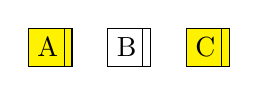
\begin{tikzpicture}
    % draw the extra path manually - works fine:
    \node[simple node, fill=yellow] at (0,0) (a) {A\,};
    \draw ([xshift=-1mm]a.north east) --([xshift=-1mm]a.south east);

    % without the fill this looks fine. (Note that "\draw node" is necessary, rather than just "\node".)
    \draw node [barred node] at (1,0) (b) {B\,};

    % but with the fill it breaks - the line is drawn behind the node instead of in front of it.
    \draw node [barred node, fill=yellow] at (2,0) (c) {C\,};
\end{tikzpicture}

\end{document}